\chapter{Theoretical background}

\label{sec:theory}

\section{Plasma modelling}
In this section, we present a short overview of the basic mathematical framework used in the study of plasma dynamics. In section \cref{subsec:basicEq}, we briefly present the equations of motion for single particle motion in electrical and magnetic fields. Then in \cref{subsec:pParam} we give an overview of essential plasma parameters.
Plasma is a collection of ionized gas, commonly referred to as the fourth state of matter. The solar wind, the polar aurorae, and lighting are some examples of plasmas that occur in nature \parencite{Chen2018}. Plasma shares many of the same properties that describe gases, but differ in being affected by magnetic and electrical fields: since plasma consists of charged particles, ions and free electrons, they are subject to the Lorentz force. The Lorentz force acting on a charged plasma particle, causes curvilinear motion further complicated by the influence of other nearby charged particles.

\section{Basic equations}

\subsection{Single particle description}
\label{subsec:basicEq}
The single particle description of a plasma describes the motion of individual charged particles moving in imposed magnetic and electrical fields. Assuming the force of gravity is sufficiently small, and assuming constant electrical and magnetic fields, the single particle motion of a charge $q$ moving at velocity $v$ in the electrical field $\vb{E}$ and magnetic field $\vb{B}$ (where bolded letters denote vector fields) is described by the Lorentz force law 

\begin{equation}\label{eq:lorentz}
    \vb{F} = q \vb{E} + q \vb{v} \cp \vb{B},
\end{equation}
where the term $q \vb{E}$ is called the Electric force, and the term $q\vb{v} \cp \vb{B}$ is called the magnetic force. When a particle moves in a static magnetic field, and no electric field is present, the particle will gyrate around magnetic field lines. Setting $E$ to zero, we have

\begin{equation}\label{eq:magF}
    \vb{F} = q \vb{v} \cp \vb{B}.
\end{equation}

The cross product of the velocity and magnetic field vector means that the magnetic force always acts perpendicularly to the direction of motion of the particle, thereby causing the particle to gyrate.

Setting the centripetal force equal to the magnitude of the Lorentz force, we can derive an expression for the gyroradius $r_g$ of the motion

\begin{equation}\label{eq:gyrorad}
    \frac{m_s v_{\perp}^2}{r_g} = \abs{q} v_{\perp} \norm{\vb{B}}
\end{equation}

Where the subscript on $m_s$ denotes the specie of the particle, and $v_\perp$ denotes the perpendicular component of velocity to the plane of $\vb{B}$. Upon rearranging, the expression for the gyroradius $r_g$ becomes

\begin{equation}
    r_g = \frac{m_s v_\perp}{\abs{q} \norm{\vb{B}}}.
\end{equation}

The particle gyrates with an angular frequency, called the cyclotron frequency $\Omega_c$, expressed as 

\begin{equation}
    \Omega_c = \frac{v_\perp}{r_g} = \frac{\abs{q} \; \norm{\vb{B}}}{m_s}
\end{equation}

The motion of a particle $q_s$ is in practical cases often modelled as the drift of the centre of gyration of the particle. When also subjected to an isotropic electrical field, this motion is called E cross B drift, or Hall drift, and can be derived from the Lorentz force equation and Newtons' second law and solving for the acceleration of the particle: If we assume the drift velocity to be constant in time, the expression for the drift $\vb{V}_D$ becomes

\begin{equation}
    \vb{V}_D = \frac{\vb{E} \cp \vb{B}}{B^2}
\end{equation}

\subsection{Kinetic description}
In the previous section, we studied the individual motion of charged plasma particles. Although the single particle description of plasma is useful in gaining an understanding in how individual particles behave in isotropic magnetic and electrical fields; it is an impractical model for analyzing macroscopic phenomena of the plasma. The introductory text "Plasma Physics: An Introduction to Laboratory, Space, and Fusion Plasmas" \parencite{Piel2017} contains a good discussion of when each plasma model should be used. The kinetic description of plasma begins with the assumption of a density distribution of charges in the six dimensional phase space varying over time. Let $f_s(\vb{x}, \vb{v}, t)$ be the continuous probability distribution, representing the probability of finding a charged particle of species $s$ at time $t$ in phase space. Multiplying the distribution of charges by the charge of the species $q_s$, and integrating over the velocity space, the charge density $\rho_s$ can be found. Summing over all the species of charge in the plasma gives us the following expression for the total charge density $\rho_c$

\begin{equation}\label{eq:rhoCharge}
    \rho_c = \sum_s q_s\int f(\vb{x}, \vb{v}, t) d^3\vb{v}.
\end{equation}

Similarly, an expression for the current density is obtained by multiplying the charge distribution by the velocity vector $v$ and integrating the result in a similar fashion to \eqref{eq:rhoCharge}

\begin{equation}
    \vb{j} = \sum_s q_s \int \vb{v} f(\vb{x}, \vb{v}, t) d^3 \vb{v}
\end{equation}


Equipped with a continuous distribution function of particles in phase-space, equations of motion that describe the flow of the charged particles can be derived from solving the Boltzmann equation. Or alternatively, when assuming a non-collisional plasma, the set of vector equations called the Vlasov equation can be used


\begin{equation}\label{eq:Vlasov}
    \pdv{f}{t} + \vb{v} \vdot \grad{f_s} + \frac{q_s}{m_s} (\vb{E} + \vb{v} \cp \vb{B}) \vdot \grad_v{f} = 0
\end{equation}

Where the operator notation $\grad_v = (\pdv{v_x}, \pdv{v_y}, \pdv{v_z})$ and $\grad = (\pdv{x},\pdv{y},\pdv{z})$ has been used. For a comprehensive derivation of the Vlasov equation see \parencite{Birdsall2004} or \parencite{Piel2017}.


\subsection{Fluid description}
In previous sections, the equations of motion for characterising plasma has been modelled by analyzing the forces acting on individual particles. While this approach can be helpful in gaining insight into the physics governing the plasma behaviour, it is difficult to apply these frameworks to practical computation models. 
\vskip 1mm
Another method, that reduces the complexity of computing individual particle motions, is treating plasma as two continuous fluids. In this approach we are able to extract macroscopic properties of the plasma, such as the density, the velocity and the mean energy. The fluid equations are derived by taking the velocity moments of the Vlasov equation \eqref{eq:Vlasov}, where the generalized velocity moment is described as

\begin{equation}\label{eq:moment}
    M^n \equiv \int f(\vb{v}) \vb{v}^n d \vb{v}
\end{equation}

The zeroth velocity moment, also called the continuity equation, can be found by multiplying equation \eqref{eq:Vlasov} by the zeroth velocity moment 

\begin{equation}\label{eq:zeromoment}
    n_s = \int f_s d \vb{v}
\end{equation}

The zeroth velocity moment for species $s$ is simply the number density for the species. Multiplying equation \eqref{eq:zeromoment} by the Vlasov equation we have

\begin{equation}\label{eq:continuity}
    \int \pdv{f_s}{t} d \vb{v} \int \vb{v} \vdot \grad{f_s} \vb{v} + \frac{q}{m} \int \vb{E} + \vb{v} \cp \vb{B} \vdot \pdv{f_s}{\vb{v}} d \vb{v} = 0
\end{equation}

With a considerable amount of manipulation \parencite[ch 7]{Chen2018}, equation \eqref{eq:continuity} reduces to

\begin{equation}\label{eq:contReduced}
    \pdv{n_s}{t} + \div{(n_s \vb{v_s})} = 0 
\end{equation}


In a similar fashion, the momentum equation can be derived from multiplying equation \eqref{eq:Vlasov} by the the first velocity moment

\begin{equation}\label{eq:firstmoment}
    M^1 = \int m_s \vb{v} f_s d \vb{v}
\end{equation}

this multiplication yields

\begin{equation}\label{eq:momentum}
     \pdv{\vb{m_s n_s v_s}}{t} + \div{\vb{P_s}} - e_s n_s (\vb{E} \ \vb{v_s} \cross \vb{B}) = \vb{F_s}
\end{equation}

Where $P_s$ denotes the pressure tensor field. The energy equation is derived from the second velocity moment

\begin{equation}
    M^2 = \int \frac{1}{2} m_s \vb{v} \vb{v} f_s d \vb{v}
\end{equation}

The second order moment described the flow of momentum, and is also called the stress tensor \parencite[Ch. 3]{Fitzpatrick2015}. Applying the second velocity moment to equation \eqref{eq:Vlasov} equation gives the partial differential equation

\begin{equation}\label{eq:energy}
    \pdv{t} (\frac{3}{2} p_s + \frac{1}{2} m_s n_s v_s^2) + \div{\vb{Q_s}} - e_s n_s \vb{E} \vdot \vb{v_s} = W_s + \vb{v_s} + \vb{v_s} + \vb{F_s}   
\end{equation}

Where the terms $\vb{Q}_s$ and $\vb{W}_s$ denote the energy flux density and total change of energy of species $s$ respectively. Equations \eqref{eq:contReduced}, \eqref{eq:momentum}, and \eqref{eq:energy}, are collectively known as the fluid equations, and written in their convective time-derivative form, can be reduced to

\begin{subequations}
    \begin{align}
        &\frac{D n_s}{D t} + n_s \div{\vb{v_s}} = 0 \\
        &m_s n_s \frac{D \vb{v_s}}{D t} + \div{p_s} - e_s n_s ( \vb{E} + \vb{v_s} \cross \vb{B}) = \vb{F_s} \\
        &\frac{3}{2} \frac{D p_s}{D t} + \frac{3}{2} p_s \div{v_s} + \vb{p_s} \colon \grad{\vb{v_s}} + \div{\vb{q_s}} = W_s
    \end{align}
\end{subequations}

Formal derivations of the fluid equations, with some differences in notation, can be found in the fundamental works of Chen \parencite{Chen2018}, and Fitzpatrick \parencite{Fitzpatrick2015}.

\subsection{Magnetohydrodynamics}
Solving the equations of motion discussed in \ref{subsec:basicEq} coupled with Maxwell's equations is extremely computationally demanding. As such, two common approximations to these equations are used, the electrostatic model, and magnetohydrodynamics.
\\
In the electrostatic approximation of plasma, the plasma currents are presumed small, thereby simplifying maxwell's equations to solving poission's equation for the electrostatic potential.
\\
In the magnetohydrodynamics, plasma is treated as a neutral yet conducting fluid. Assuming a quasi-neutral, plasma at thermodynamic equilibrium Maxwell's equations \parencite[Ch. 9-9-1]{Hockney1988} reduce to

\begin{subequations}
    \begin{align}
        \nabla \cross \vb{B} &= \mu_0 \vb{j} \\
        \nabla \cross \vb{E} &= - \pdv{\vb{B}}{t} \label{eq:curlE}\\
        \nabla \cdot \vb{B} &= \nabla \cdot \vb{E} = 0    
    \end{align}
\end{subequations}

The force equation can then be rewritten in terms of current density $\vb{j}$ and the conductivity $\sigma$ as

\begin{equation}\label{eq:maghydroCurr}
    \vb{j} = \sigma (\vb{E} + \vb{v} \cross{B})    
\end{equation}

From the assumption of a perfectly conducting fluid, and finite current density $\vb{j}$, then 

\begin{equation}\label{eq:magHydroInf}
    \vb{E} + \vb{v} \cross \vb{B} = 0
\end{equation}

 From equation \eqref{eq:magHydroInf}, equation \eqref{eq:curlE} reduces to

\begin{equation}
    \pdv{\vb{B}}{t} = \nabla \cross (\vb{v} \cross \vb{B})
\end{equation}

The equations must then be closed using the fluid continuity equations and the momentum balance equations

\begin{subequations}
    \begin{align}
        \pdv{\rho}{t} &= \nabla \cdot (\rho \vb{v}) \\
        \rho \dv{\vb{v}}{t} &= \grad{p} + \vb{j} \cross \vb{B}
    \end{align}
\end{subequations}

Where $\rho$ is the fluid density, $p$ is the fluid pressure, and $\dv{\vb{v}}{t}$ is the material derivative, i.e the rate of change of with respect to the moving fluid particle.


\section{Plasma parameters}\label{subsec:pParam}
In this section, the basic parameters used in the analysis and simulation will be introduced. We discuss the notion of a plasma temperature, present the characteristic length and frequency scales the Debye length, and plasma frequency. Additionally, we discuss the principle of quasineutrality in relation to plasma. 

\subsection{Temperature}\label{subsec:temperature}
The temperature of a plasma is a measure of the average kinetic energy of the individual species that make up the plasma. For a mono-atomic gas, with a probability distribution $f(u)$, Chen \parencite[Section 1.3]{Chen2018} gives the following equation for the average kinetic energy

\begin{equation}\label{eq:avgEint}
    E_{av} = \frac{\int^\infty_{-\infty} \frac{1}{2} m u^2 f(u) du}{\int^\infty_{-\infty} f(u) du}
\end{equation}


By defining the variables 

\begin{equation*}
    v_{th} \equiv (2 K T / m)^{\frac{1}{2}} \hspace{10pt} \text{and} \hspace{10pt} y \equiv \frac{v_{th}}{u}
\end{equation*}
    
and integrating the numerator by parts, equation \eqref{eq:avgEint} reduces to

\begin{equation}\label{eq:avgE1D}
    E_{av} = \frac{1}{2} K T
\end{equation}

Where $K$ denotes the Boltzmann constant. Chen extends this argument for particles with three degrees of freedom. Integrating Maxwell's distribution in three dimensions in a similar fashion to \eqref{eq:avgEint} and cancelling the integrals, the average kinetic energy is

\begin{equation}\label{eq:avgE3D}
    E_{av} = \frac{3}{2} K T
\end{equation}

In plasma physics, it is common to use average energy rather than temperature as they are so closely linked. Calculations are often reduced in complexity by using the electron volt as the basic units of energy. It is defined as the amount of energy required to move a single electron across an electrical potential difference of 1 volt. One eV is therefore approximately equal $1.6 \text{x} 10^-19$ J, with a conversion factor to temperature, in Kelvin

\begin{equation*}
    1 eV \approx 11600 K
\end{equation*}

\subsection{Debye length}
The Debye length is a parameter that measures the net persistence of the electrostatic effect of a charged particle. This effect is also known as Debye shielding, \parencite[Section 3.1.2]{HutchinsonIanH2002Popd} presents a definition for the Debye length by analyzing the potential profile of a test charge placed in a cold plasma. In a non isothermal plasma ions can be assumed to be stationary in relation the more energetic electrons. The electrons density is then determined from the Boltzman factor

\begin{equation}\label{eq:boltzmannFactor}
    n_e = n_{\infty} \exp(\frac{e \phi}{T_e})
\end{equation}

Where $T_e$ denotes the electron temperature, $n_{\infty}$ is the density of electrons far away from the perturbing test charge, and where $\phi$ is the electrical potential as a function of the radial distance from the test function. Inserting equation \eqref{eq:boltzmannFactor} into Poisson's equation;

\begin{equation}\label{eq:poissonDebye}
    \laplacian{\phi}  = - \frac{\rho}{\epsilon_0} = \frac{-e}{\epsilon_0} (n_i - n_e) = \frac{-e}{\epsilon_0} n_{\infty} \left[1 - \exp (\frac{e \phi}{T_e}) \right]
\end{equation}

Assuming $e \phi \lll T_e$, then it is reasonable to only keep the linear terms of the Taylor expansion of the $\exp (\frac{e \phi}{T_e})$ term on the right hand side of equation \eqref{eq:poissonDebye}. Poisson's equation then takes the form of Helmholtz equation

\begin{equation}\label{eq:poissonSimple}
    \laplacian{\phi} - \frac{1}{\lambda_D^2} \phi = 0
\end{equation}


Where the Debye length $\lambda_D$ has been defined as follows:

\begin{equation}\label{eq:Helmholtz}
    \lambda_d \equiv \sqrt{\frac{\epsilon_0 k T_e}{n_e e^2}}
\end{equation}

The solution of equation \eqref{eq:poissonSimple} takes the form

\begin{equation*}
    V \propto \exp (\frac{\pm x}{\lambda_D})
\end{equation*}

The Debye length is then a measure of the shielding distance or thickness of the sheath that forms around a charged object embedded in a plasma \parencite[Section 1.4]{Chen2018}.


\subsection{quasineutrality}
Now that we have presented an expression for the Debye length, the approximation of quasineutral plasma can be defined: When the length scale of interest is much smaller than the Debye length, i.e $\lambda_D \lll L$, the density of ions is approximately equal to the density of electrons \parencite[Section 1.4]{Chen2018}. Or in other terms

\begin{equation}
    n_i \approx n_e \approx n
\end{equation}

Where n is a common density called the plasma density. When this approximation holds, the plasma is said to be quasineutral. Note that this approximation still allows for variations in charge at smaller length scales than $\lambda_D$. 

\subsection{Electron plasma frequency}
In plasma simulations of the solar wind an important physical phenomena is plasma oscillation, otherwise called Langmuir waves. In a neutral plasma, disturbances in the density of electrons (and ions) cause oscillations due to the restorative Coulomb force. For solar wind, and other cold plasmas, the frequency of the oscillations of electrons are expressed as

\begin{equation}\label{eq:plasmaFreq}
    \omega_{pe} = \sqrt{\frac{n_e e^2}{\epsilon_0 m_e}}
\end{equation}

$\omega_{pe}$ is called the electron plasma frequency. A similar expression exists for the oscillations of ions, but due to their higher mass they oscillate much slower rate than the electrons. Equation \eqref{eq:plasmaFreq} is formally derived from Maxwell's equations \parencite{Fitzpatrick2015}, \parencite{HutchinsonIanH2002Popd} by assuming an infinite plasma not affected by an external magnetic field, no thermal motion i.e $KT = 0$, and ion fixed in space  in a uniform distribution \parencite[Section 4.3]{Chen2018}.



\section{The solar wind plasma environment}
In this section, a brief overview of the physics and basic plasma parameter values of the solar wind are presented. These data will be necessary in building the computational parameters required for the charging simulations of space probes moving in the interplanetary medium presented later in this thesis.
\\
The solar wind is a non-isothermal plasma with a temperature averaging around 10 $eV$, that is primarily composed of free electrons, ions and alpha particles. The density of the solar wind plasma is relatively low as compared to other naturally occurring plasmas with a mean value of around 5 $cm^{-3}$. It flows with a drift velocity ranging from 400 $km/s$ up to 900 $km/s$ during periods of high solar activity \parencite{LAI2019}. In close proximity to the sun, the solar wind density increases significantly, potentially charging space probes to values as low as hundreds of volts \parencite{LAI2019}, \parencite{Deca2013}, \parencite{Garrett1981}.


\todo{Check if I am allowed to use an image from copyrighted works!}
%\begin{figure}[h!]
%    \centering
%    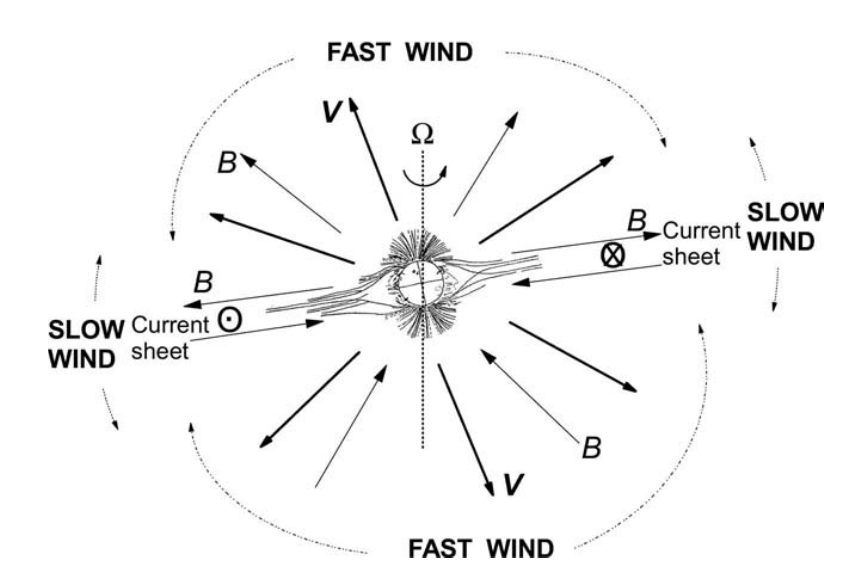
\includegraphics[scale=0.65]{figures/solarWind.png}
%    \caption{Large-scale structure of the solar wind}
%    \label{fig:solarWind}
%\end{figure}

\subsection*{Interactions with solar system objects}
The properties of the solar wind can change significantly in regions in close proximity to solar system objects. Planets with internal magnetic fields, will cause magnetohydrodynamic (MHD) shock formation \parencite{Luhmann2004}, \parencite{Benna2009}, and bodies without an intrinsic magnetic field may still affect the flow of the solar wind plasma due to induced magnetic fields from solar wind charge collection or interaction with the ionosphere of the body.

\begin{figure}
\centering
\begin{subfigure}{.5\textwidth}
    \centering
    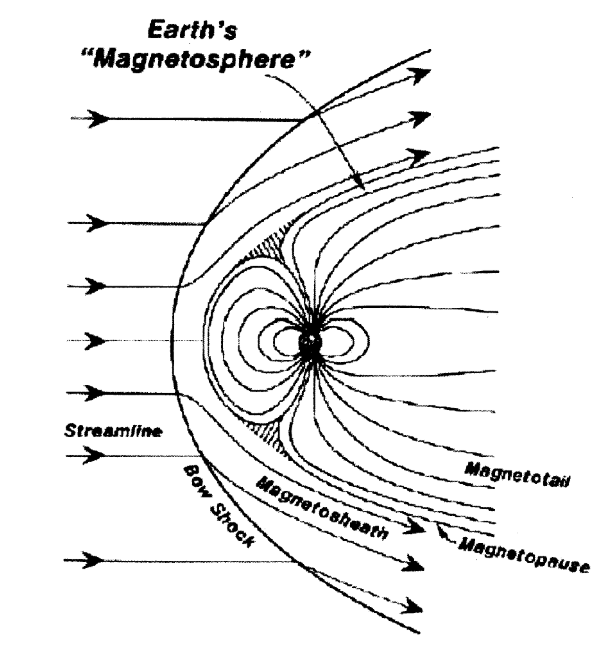
\includegraphics[width=\linewidth]{figures/EarthMagnetosphere.PNG}
    \caption{Magnetosphere of Earth}
    \label{fig:EarthMagSph}
\end{subfigure}%
\begin{subfigure}{.5\textwidth}
    \centering
    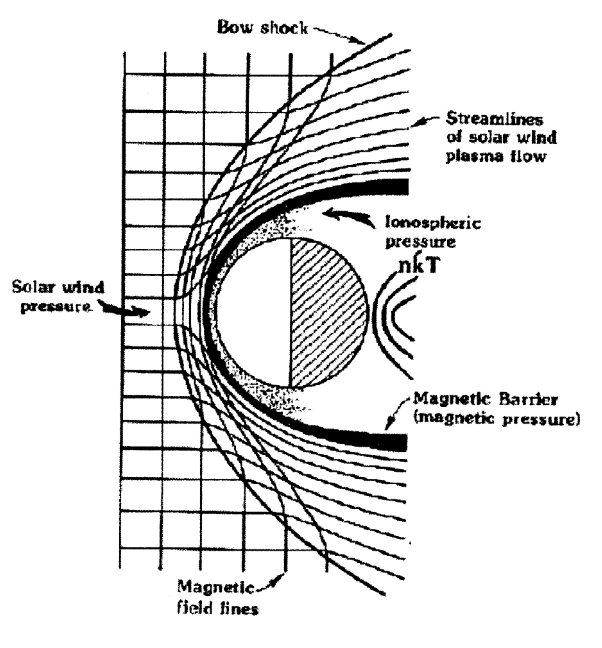
\includegraphics[width=\linewidth]{figures/inducedMagnetosphere.PNG}
    \caption{Induced magnetosphere on Venus}
    \label{fig:VenusMagSph}
\end{subfigure}
\caption{Differences in magnetosphere structures for bodies with and without internal magnetic fields, reproduced from }
\label{fig:magnetosphere}
\end{figure}

Figure \ref{fig:magnetosphere} shows the basic structure, and differences, in the magnetospheres of two bodies with and without internal magnetic fields. This thesis is concerned with simulating the charging characteristics of the BepiColombo satellite, the MMO (Mercury Magnetospheric Orbiter). Mercury has an intrinsic, yet relatively weak, magnetic field. 
\\
As such, figure \ref{fig:EarthMagSph} is illustrative of the magnetic environment the MMO spacecraft will be subjected to. The bow-shock forms due to the compression of the solar wind from the obstruction of the magnetosphere of the body in question, the shocks location and properties changes dynamically depending on the pressure exerted by the solar wind. Immediately behind the bow-shock is the region called the magnetosheath. In this region the charged particles have a lower density yet higher average temperature than that of the solar wind \parencite{Benna2009}. 
\\
Separating the magnetosphere of the earth, or Mercury, is the magnetopause. The magnetopause is defined as the region around an object where the dynamic pressure of the solar wind balances with the pressure from the intrinsic magnetic field of the object. Beyond the magnetopause, the intrinsic magnetic field of the planet dominates. In this region charged plasma particles move in spirals following magnetic field lines of the planet, the magnetosphere of Earth also contains a region of high density cold plasma called the plasmasphere. The composition of the plasma, its temperature and density in these regions vary significantly. The charging of a spacecraft will then vary significantly as a spacecraft orbits a planet, and it is therefore important to determine the location of these regions with respect to the planet. 
\\
The location of the magnetopause of a planet with an intrinsic field can be approximated by substituting the distance of the magnetopause $r_M$ into the balance expression for the planets magnetic field strength. Balancing the dynamic pressure of the sun with the magnetic pressure \parencite{Meyer-Vernet2007}, we have

\begin{equation}\label{eq:pBalanceRough}
\rho_w v^2_w \sim B^2_{\mu} / 2 \mu_0  
\end{equation}
Where $\rho_w$ and $v_w$ is the solar wind density and velocity respectively, $B_{\mu}$ is the dipole magnetic field strength, and $\mu_0$ is the vacuum permeability. The magnetic field strength is expressed as

\begin{equation}\label{eq:magFieldStrength}
    B_{\mu} = (\mu_0 / 4 \pi) \mu / r^3_M
\end{equation}

where $\mu$ is the permeability of the planet. However, the magnetopause must carry a current to confine the planets dipole magnetic field. This current produces a magnetic field on the order of magnitude to $B_{\nu}$. Therefore, just inside the magnetopause, the magnetic field strength is approximately twice $B_{\nu}$. The balance equation \eqref{eq:pBalanceRough} then becomes 

\begin{equation}\label{eq:pressureBalance}
    \rho_w v^2_w \approx \frac{(2 B_{\mu})^2}{2 \mu_0} 
\end{equation}

Substituting in the magnetic field strength from equation \eqref{eq:magFieldStrength} the distance of the magnetopause on the sun-ward side to the planet is approximately 

\begin{equation}\label{eq:magnetopause}
    r_M \approx \left(\frac{\mu}{4 \pi} \sqrt{\frac{2 \mu_0}{\rho_w v^2_w}} \right)^{\frac{1}{3}}
\end{equation}

This can be expressed as a relative distance by introducing the radius of the planet $R$ and the magnetic field strength at the equator $B_0 = (\nu_0 / 4 \pi) \nu / R^3$

\begin{equation}
    \frac{r_m}{R} \approx \left(\frac{2 B^2_0}{\nu_0 \rho_w v^2_w} \right)^{1/6}
\end{equation}


In her book \parencite{Meyer-Vernet2007}, Meyer-Vernet also gives an approximation for the distance from the planet to the bow-shock by assuming a conical function describing the radius $r$ from the foci (the planet) to the bow shock. The radius $r$ on the line extending from the planet to the sun is approximately

\begin{equation}
    r \simeq (1 + \epsilon) \, r_M
\end{equation}

Where $\epsilon$ is the eccentricity of the conic section. Typically this value is around $\epsilon \simeq 0.5$.

\section{Spacecraft charging in plasma}
A spacecraft collects charged particles when moving relatively to ambient plasma, this change in net charge on the spacecraft causes an electrical field according to Gauss's Law \parencite[Ch. 1]{LAI2019}. When the charging of the spacecraft reaches a non-oscillatory steady state, the sum of currents from all the species in the plasma is zero, and the net charging is constant. This is expressed as 

\begin{equation} \label{eq:currentBalance}
    \dv{Q}{t} = \sum_s I_s(V) = 0
\end{equation}

The solution of equation \eqref{eq:currentBalance} for $V$ is called the floating potential of the spacecraft, and is relative to the neutral plasma. The floating potential of a spacecraft in a drifting plasma is usually negative, since the electrons move at a higher speed than the ions.
\\
For complex geometries it is non-trivial to find analytical expressions for the currents $I_s$ charging the spacecraft; in this section, Langmuir probe theory and orbital motion-limited theory is discussed as the basic tools for analyzing spacecraft charging with simple geometries. The primary charging mechanisms that effect the overall potential of a spacecraft are then presented. Special attention is given to the photoelectric effect and the spacecraft photoelectric current, as the implementation of this current in a computational model is the overall objective of this thesis \todo{clunky?}.


\subsection{Langmuir probe theory}
A Langmuir probe is a simple device used in the laboratory to measure the temperature, the density, and the electrical potential of a plasma. A Langmuir probe consists of one or more, often spherical, electrodes inserted into the ambient plasma. Either a time varying or constant potential is induced between the electrodes, or between the electrodes and some electrical ground, causing the probe to collect charged particles. By analysing the current $I(V)$ for different potentials, the properties of the surrounding plasma can be extracted  \parencite{Garrett1981}, \parencite{LAI2019}, \parencite{Miloch2012}. When immersed in a plasma, a spacecraft behaves in a similar fashion to a Langmuir probe. The difference is that in the case of a spacecraft a potential is not applied, but can be measured as a response to incoming and outgoing currents \parencite[Ch. 2]{LAI2019}. 


\subsection*{Orbital motion-limited theory}
In orbital motion limited theory, or OML theory for short, the charge flux impinging on a spacecraft is determined from the conservation of energy and angular momentum of species travelling in proximity to a spacecraft \parencite{LAI2019}, \parencite{Garrett1981}. From conservation of energy, an expression for the impact velocity on a spherical spacecraft can be obtained, and from conservation of momentum an expression for the distance from the centre of the spacecraft to the straight line of travel can be found. In \parencite[Ch. 2.1]{LAI2019} these expressions are given as 

\begin{subequations}
    \begin{align}
        v_a &= v_{th} \left(1 - \frac{q \phi}{kT} \right) \label{eq:impactvel} \\
        h &= a \left(1 - \frac{q \phi}{kT} \right) \label{eq:distStraight}
    \end{align}
\end{subequations}

Integrating the particle distribution $f_s(\vb{x}, \vb{v}, t)$ using equation \eqref{eq:impactvel} and \eqref{eq:distStraight} as limits of integration, we can find the flux of particles that impact the spacecraft. It is often convenient work with a normalized potential variable in the formulas for current, define

\begin{equation}\label{eq:normPot}
    \eta_s \equiv - \frac{q_s V}{k T_s}
\end{equation}

Using the normalized potential, particles with $n_s < 0$ will be repelled, and particles with $n_s > 0$ will be attracted to the spacecraft \parencite{Marholm2019}. Expressions for the integration of the particle distribution has been found for some simple geometries, for species with $n_s > 0$ with the assumption of a plasma with no internal magnetic field and zero drift, by Mott-Smith and Langmuir \parencite{Mott-Smith1926}

\begin{subequations}
    \begin{align}
        I_s (\eta_s) &= I_{th,s} \label{eq:IPlane} \\
        I_s (\eta_s) &= I_{th,s} \left(\frac{2}{\sqrt{\pi}} \sqrt{\eta_s} + \exp(\eta_s) \hspace{2pt} \text{erfc}(\sqrt{\eta_s}) \right) \label{eq:ICylinder}\\
        & \approx I_{th,s} \frac{2}{\sqrt{\pi}} \sqrt{1 + \eta_s} \\
        I_s(\eta_s)  &= I_{th,s} (1 + \eta_s) \label{eq:Isphere}
    \end{align}
\end{subequations}

Where equations \eqref{eq:IPlane}, \eqref{eq:ICylinder} and \eqref{eq:Isphere} are the functions of current for a plane, a cylinder, and a sphere respectively. These functions are derived based on the assumption that the cylinder is long compared to $\lambda_D$, the radius of the sphere and the cylinder to be small compared to $\lambda_D$, and the plane to be wider than $\lambda_D$. The notation $I_{th}$ is used to denote the current collected when the object is neutrally charged, i.e $\eta_s = 0$, and $erfc(\sqrt{\eta_s})$ is the complementary error function defined as

\begin{subequations}
    \begin{align*}
        \text{erfc}(z) &\equiv 1 - \text{erf}(z) \\
        &= \frac{2}{\sqrt{\pi}} \int^\infty_z e^{-t^2} dt
    \end{align*}
\end{subequations}


\subsection*{The photoemission current}\todo{Includes discussion on Blackbody radiation..}
In 1921, Albert Einstein was awarded the Nobel price in physics for his discovery of the mathematical law governing the photoelectric effect \parencite{NobelMediaAB}. Qualitatively, the photoelectric effect occurs when a quantum of light, a photon, is absorbed by an electron in some material causing its energy to exceed the binding energy of that material and being ejected from the surface of the material. This binding energy of the material is called the work function of the material. Mathematically, with differences in notation \parencite{Einstein1905}, Einstein's law is expressed as

\begin{equation}\label{eq:phelectron}
    E = h \nu - W
\end{equation}

Where $E$ denotes the maximum kinetic energy of the ejected electron, $h$ is Planck's constant, $\nu$ is the wavelength of the light quanta, and $W_f$ denotes the work function of the material. It is often useful in engineering to express equation \eqref{eq:phelectron} in terms of the threshold frequency $\nu_0$ at which the photons have enough energy to cause photoemission. Using the relation $E = W_f = h \nu_0$, equation \eqref{eq:phelectron} becomes

\begin{equation}\label{eq:phfreq}
    E_{k} = h(\nu - \nu_0)
\end{equation}

From equation \eqref{eq:phelectron}, it is evident that the photoelectron yield is dependent on the material composition of the spacecraft. Table \ref{tab:workfunc} shows the work functions for some of the materials commonly used in space applications, these data have been reproduced from \insertref{Handbook of Chemistry and Physics} and \insertref{Experimental Investigation of Photoemission from Satellite Surface Materials}.

\begin{table}[h!]
    \centering
    \begin{tabular}{|c|c|}
        \hline
        \textbf{Material} & \textbf{Work function (eV)} \\ \hline
        Aluminium         & 4.0                    \\ \hline
        Gold              & 4.2                    \\ \hline
        Silver            & 4.62                   \\ \hline
        Stainless steel   & 4.4                    \\ \hline
        Graphite          & 4.7                    \\ \hline
    \end{tabular}
    \caption{Work function for common materials used in space applications}
    \label{tab:workfunc}
\end{table}

With an expression for the minimum frequency below which photoemission occurs it possible to compute the photoelectron current; defining a photoelectron yield $Y(\omega)$  (photoelectrons per photon at some energy $\omega$) as

\begin{equation} \label{eq:naivePhYield}
    Y(w) = 
    \begin{cases}
        1 \quad& if \quad \omega > h \nu_0 \\
        0 \quad& if \quad \omega \leqslant h \nu_0
    \end{cases}
\end{equation}


Then, the photoelectron current flux $J_{ph}$ can be found by integrating over the energy of the incoming photons \insertref{Fundamentals of sc, ch 7}

\begin{equation}\label{eq:phCurrentNaive}
    J_{ph} = \int^\infty_0 Y(\omega) f_s(\omega) \, d\omega
\end{equation}


Strictly speaking, equation \eqref{eq:naivePhYield} is only an approximation for the yield of photoelectrons. A more accurate description has to account for the amount of photons reflected from the surface, thereby not contributing to the total photoelectron current flux. Defining the reflectance of the surface exposed to sunlight as $R(\omega)$, equation \eqref{eq:phCurrentNaive} becomes \insertref{Fundamentals of sc charging, ch 7}

\begin{equation}\label{eq:phCurrentR}
    J_{ph}(R) = \int^\infty_0 Y(\omega, R) f_s(\omega) \, d\omega
\end{equation}

Both the photoelectron yield, and the reflectance of the spacecraft material is additionally dependent on the incident angle $\theta$ of the surface to the direction of travel of the photons. Lai gives the following equation \insertref{} for current flux $J_{ph}(\theta)$ when incidence angle is accounted for

\begin{equation}\label{eq:phCurrentFull}
    J_{ph}(\theta) = \int^\infty_0 f_s(\omega) Y^{*}[\omega, R(\omega, \theta)][1 - R(\omega, \theta)] \cos \theta \; d\omega
\end{equation}

Where $Y^{*}(\omega, R(\omega, \theta))$ is the photoelectron yield per \emph{absorbed} photon. Using estimates for terms $Y^{*}$ and $1 - R(\omega, \theta)$ and cancelling cosine terms in the product, equation \eqref{eq:phCurrentFull} becomes

\begin{subequations}
    \begin{align}
        J_{ph}(\theta) &= \int^\infty_0 f_s(\omega) Y(\omega)(1 - R(\omega)) \cos \theta \; d\omega \\
        J_{ph}(\theta) &= J_{ph}(0) \cos \theta
    \end{align}
\end{subequations}


Finally, the photoelectron current $I_{ph}(\theta)$ can be expressed as 

\begin{equation}\label{eq:phCurrent}
    I_{ph}(\theta) = J_{ph}(0) A \cos \theta 
\end{equation}

Where $A$ is the surface area of the spacecraft exposed to sunlight. Inserting equation \eqref{eq:phCurrent} into equation \eqref{eq:currentBalance}, and with a known photon flux from blackbody radiation theory, the floating potential for a spacecraft subject to photoelectric and ambient plasma charging can be computed.

\subsubsection*{The sun as a blackbody radiation source}
In the previous section, an expression for the photoelectron current was shown. If we are to compute the floating potential of a spacecraft, it is necessary to either know the value of the photoelectron current a priori or to compute its value based on the amount of photon flux through the spacecraft surface. In this section we discuss the theory of blackbody radiation as a method of computing solar photon flux.
\\
A blackbody is an object in thermodynamic equilibrium that absorbs all frequencies of radiation, without reflecting any of the incoming radiation\insertref{Kirchhoff, 1860, Annalen der Physik und Chemie}. In Planck's seminal paper on the theory of heat radiation, Planck gives the following three conditions that a blackbody must satisfy \insertref{Planck, The theory of heat radiation, translation, p10.}

\begin{quote}
    First, the body must have a black surface in order to allow the incident rays to enter without reflection. [...] Second, the black body must have a certain minimum thickness depending on its absorbing power, in order to insure that the rays after passing into the body shall not leave it again at a different point of the surface. [...] Third, the black body must have a vanishingly small coefficient of scattering. Otherwise the rays received by it would be partly scattered in the interior and might leave again through the surface
\end{quote}

The sun does not perfectly absorb all frequencies of electromagnetic radiation, and neither is it in perfect thermodynamic equilibrium; sunspots have a measurably lower temperature than the surrounding photosphere \insertref{The
observations also suggest that the coronal temperature above sunspots is lower than in
their surroundings, Sunspots: An overview}. However, energy absorbed and emitted by the sun is in steady state and can therefore be approximated as a black body radiator. 
//
In "The theory of heat radiation" Planck derives the following expression for the energy density of the electromagnetic radiation emitted by a blackbody  

\begin{equation}\label{eq:planckFreq}
    B(\nu, T) = \frac{2 h \nu^3}{c^2} \frac{1}{\exp(\frac{h \nu}{k_B T}) - 1}
\end{equation}

Where $\nu$ is the frequency of the electromagnetic radiation emitted, $T$ is the temperature of the blackbody measured in Kelvin, $c$ is the speed of light, $h$ is the planck's constant, and $k_b$ is the Boltzmann constant. Equation \eqref{eq:planckFreq} is called Planck's law, and can be similarly expressed in terms of the wavelength of the radiation $\lambda$.

\begin{equation}\label{eq:planckWave}
    B(\lambda, T) = \frac{2 h c^2}{\lambda^5} \frac{1}{\exp(\frac{hc}{\lambda k_B T}) - 1}
\end{equation}

The spectral energy computed from the equations above can be expressed in many units depending on the problem at hand. Of particular interest in this thesis is expressing the spectral energy as the number of photons emitted at a particular wavelength. In the derivation of Planck's law; Planck is often credited as the father of modern quantum mechanics by historians for his idea that the radiation emitted by a blackbody at certain frequencies as packets of energy \insertref{a historical text on the history of quantum mechanics, i.e }

Figure \ref{fig:blackbody} plots the irradiance given by equation \eqref{eq:planckWave} for some values of $T$, the suns radiative output can be approximated by assuming a blackbody temperature $T \approx 5800 K$, shown in the figure as a blue line.

\begin{figure}[h!]
    \centering
    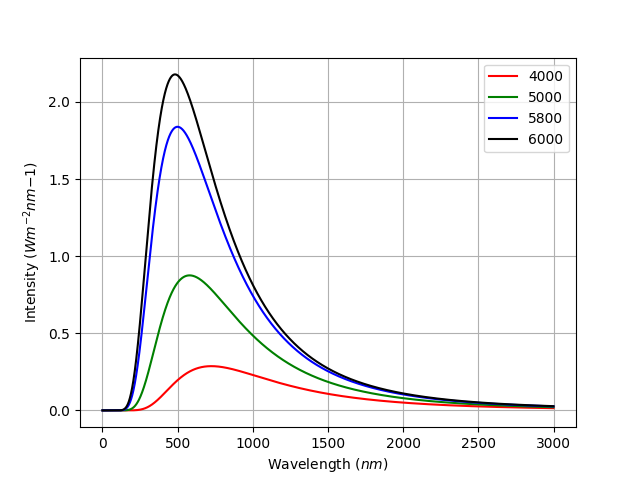
\includegraphics[scale=0.6]{figures/blackbody.png}
    \caption{Irradiance of blackbody radiation for different temperatures}
    \label{fig:blackbody}
\end{figure}


The radiation calculated from equation \eqref{eq:planckFreq} is commonly given in the units $W m^{-2} Sr^{-1} nm^{-1}$, called spectral radiance, it is the radiance of a surface per unit wavelength. In figure \ref{fig:blackbody}, the radiance is multiplied by the ratio $\frac{R_{\odot}}{a_{\oplus}}$ (where $R_{\odot}$ is the radius of the Earth, and $a_{\oplus}$ is the solar radius) to give the spectral irradiance as measured on earth, the units then are given as  $W ^{-2} m^{-2} nm^{-1}$.
\\
\insertref{The solar reference spectrum in April 2008 as recorded by the Solar instrument on the International Space Station. \url{https://www.esa.int/ESA_Multimedia/Images/2017/12/Solar_spectrum}}

\begin{figure}
    \centering
    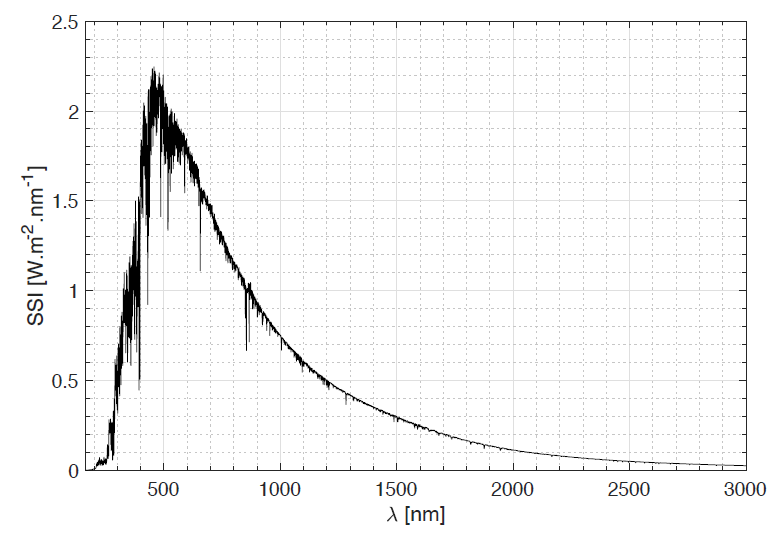
\includegraphics[scale=0.6]{figures/solarspectrum.png}
    \caption{Solar irradiance as measured onboard the International Space Station}
    \label{fig:solIrradiance}
\end{figure}

\newpage

Comparing figure \ref{fig:blackbody} to figure \ref{fig:solIrradiance}, it can be seen that aside from smaller fluctuations in electromagnetic radiation, due to absorption of energy at certain frequencies in the solar atmosphere, our approximation of the sun as a blackbody emitter is a good one. 
\\
Given the work function (or more accurately, the cut-off wavelength or frequency) of the material of a spacecraft, and assuming a photoelectron yield of one photoelectron to one photon under the cut-off wavelength, integrating equation \eqref{eq:planckWave} gives the photoelectron flux emitted by the surface of a spacecraft exposed to sunlight. Integrating planck's law for a given frequency band is non-trivial, in \ref{sec:methods}, the method for integrating Planck's law by Widger and Woodall \insertref{Integration of Planck blackbody radiation function, Widger \& Woodall} is presented in detail. 


\subsection*{Secondary and backscattered electrons}
Secondary and backscattered electrons can, depending on the ambient plasma environment and the material properties of the spacecraft in question, contribute significantly to the overall charge of a spacecraft. Both secondary and backscattered electrons provide a source of outgoing electrons from surfaces \insertref{Fundamentals of sc charging}. 
\\
At higher electron temperatures, the electrons impinging on a spacecraft may have high enough energy to interact with the electrons embedded in the surface material thereby releasing one or more electrons from the surface. The yield of secondary electron emission, or probability of emission, is a function of energy and is denoted as $\delta(E)$. 
\\
In a finite range ambient electron temperature, certain materials $\delta(E)$ can exceed one; gold, aluminum oxide, and Kapton are some common materials used in spacecraft for which $\delta(E)$ exceeds one \insertref{Fundamentals of sc charging}. When $\delta(E) > 1$ there is a net total flux of outgoing electrons thereby causing the spacecraft to charge positively.  
\\
Since the outgoing flux of electrons are dependent on the incoming electrons, one can calculate the secondary electron flux based on the incoming electron distribution $f(E)$. The current flux equation for secondary electrons is then

\begin{equation}\label{eq:secondaryE}
    j_s = \int^{\infty}_0 \delta(E) f(E) dE
\end{equation}


Backscattered electron emission is similar to secondary electron emission in that the mechanisms are dependent on incoming electrons from the ambient plasma. An electron is backscattered due to an inelastic collision with some surface material. 
\\
The outgoing electron is the same electron that collided with the surface material, backscattering of electrons can then be thought of as a form of reflection. Since the outgoing and incoming electron is the same particle, the probability of backscattering, $\eta(E)$, cannot exceed 1. 

Similarly to the secondary electron emission mechanism, the backscattering effect is dependent on the distribution of the electrons in the ambient plasma, so a similar integral to equation \eqref{eq:secondaryE} can be formed for the backscattered electron current flux 

\begin{equation}\label{eq:backscatterE}
    j_b = \int^{\infty}_0 \eta(E) f(E) dE
\end{equation}

\subsection*{Artificial sources of spacecraft charging}
Artificial sources of charging can occur both as a method for charge mitigation on spacecraft, as well as an adverse side effect of charged particle emitting equipment onboard. The SCATHA spacecraft launched by NASA was one of the first flown mission that successfully proved that spacecraft could be discharged safely without damaging scientific instruments \insertref{SCATHA}. 
\\
Charge mitigation methods can be subdivided into active and passive methods, the difference being passive methods require no control mechanisms and are automatic, whereas active mitigation requires some form of control system. These systems can be further subdivided into where the discharging occurs, whether it is on the spacecraft frame or dielectric surfaces.
\\
One of the simplest methods for discharging a spacecraft is by using a simple sharp spike protruding from the spacecraft surface. Since the radius of curvature is small at the tip of the spike, a large electrical field is generated causing electron emission from the tip. The flux of outgoing electrons reduces the negative potential the spike is connected to. Lai \insertref{A critical overview on spacecraft charging mitigation methods, 2003} gives the following equation, with differences in notation, for the current flux of a sharp spike 

\begin{equation}
    j_{spike} = A E^2 \exp \left(- \frac{B W^{\frac{3}{2}}}{E} \right)
\end{equation}

Where A and B are some constant, E is electric field strength and W is the surface material work function.
\\
Not all sources of artificial charging are beneficial however, ion engines expel high density plasma that may return to the already charged surfaces of the spacecraft. Differential charging between conducting and dielectric surfaces can occur in this case, causing damage to onboard electrical equipment. Deriving analytical expressions for charging due to electrical thrusters is impractical, and is typically simulated; \insertref{bepiColombo plasma simulation} shows one such simulation of the mercury transfer module thruster on the BepiColombo spacecraft. 